%------------------------------------%
%----- 4_Versuchsergebnisse.tex -----%
%------------------------------------%
%------------------------------------%
%
\subsection{Messdaten}
\label{subsec:4_Daten}
%
Der Stromfluss durch die Schaltung wurde über das Ohmsche Gesetz am Widerstand $R$ bestimmt:
%
\begin{align*}
  I_\mathrm{pp} = \frac{U_\mathrm{R,pp}}{R}
  \numberthis
  \label{eq:4_I}
\end{align*}
%
Der Betrag der Gesamtimpedanz $Z_\mathrm{ges}$ ergibt sich als Quotient aus dem Spitze-Spitze-Wert der Eingangspannung, $U_\mathrm{E,pp}$, und dem Spitze-Spitze-Wert des Stromes, $I_\mathrm{pp}$:
%
\begin{align*}
  Z_\mathrm{ges} = \frac{U_\mathrm{E,pp}}{I_\mathrm{pp}}
  \numberthis
  \label{eq:4_Z}
\end{align*}
%
Die Messergebnisse sind in Tab. \ref{tab:4_Messdaten} und \ref{tab:4_Messdaten_2} dargestellt\footnote{Alle Werte aufgenommen bzw. berechnet von \autorA}.
%
\begin{table}[H]
  \small
  \centering
	\caption{Messergebnisse}
	\label{tab:4_Messdaten}
	\begin{tabular}{rrrrr}
	  \toprule
		%
	  \multicolumn{1}{c}{Einstellwerte} &
		\multicolumn{2}{c}{Messwerte} &
		\multicolumn{2}{c}{Berechnete Werte} \\
		\cmidrule(lr{1mm}){1-1}\cmidrule(lr{1mm}){2-3}\cmidrule(lr{1mm}){4-5}
		%
		$f_\mathrm{E}$ in \si{\kilo\hertz} &
		$U_\mathrm{E,pp}$ in \si{\volt} &
    $U_\mathrm{R,pp}$ in \si{\volt} &
    $I_\mathrm{pp}$ in \si{\milli\ampere} &
		$\left|\underline{Z}_\mathrm{ges}\right|$ in \si{\kilo\ohm}\\
		\midrule
		%
    \input{src/4_Messdaten_1-65.txt}
    %
		\bottomrule
	\end{tabular}
\end{table}
%
\begin{table}[H]
  \small
  \centering
	\caption{Messergebnisse (Forts.)}
	\label{tab:4_Messdaten_2}
	\begin{tabular}{rrrrr}
	  \toprule
		%
	  \multicolumn{1}{c}{Einstellwerte} &
		\multicolumn{2}{c}{Messwerte} &
		\multicolumn{2}{c}{Berechnete Werte} \\
		\cmidrule(lr{1mm}){1-1}\cmidrule(lr{1mm}){2-3}\cmidrule(lr{1mm}){4-5}
		%
		$f_\mathrm{E}$ in \si{\kilo\hertz} &
		$U_\mathrm{E,pp}$ in \si{\volt} &
    $U_\mathrm{R,pp}$ in \si{\volt} &
    $I_\mathrm{pp}$ in \si{\milli\ampere} &
		$\left|\underline{Z}_\mathrm{ges}\right|$ in \si{\kilo\ohm}\\
		\midrule
		%
    \input{src/4_Messdaten_66-1000.txt}
    %
		\bottomrule
	\end{tabular}
\end{table}
%
%
%
\newpage
\subsection{Ergebnisplots}
\label{subsec:4_Plots}
%
%------------------------------%
%----- Beginn eures Teils -----%
%------------------------------%
%
\begin{figure}[H]
    \centering
    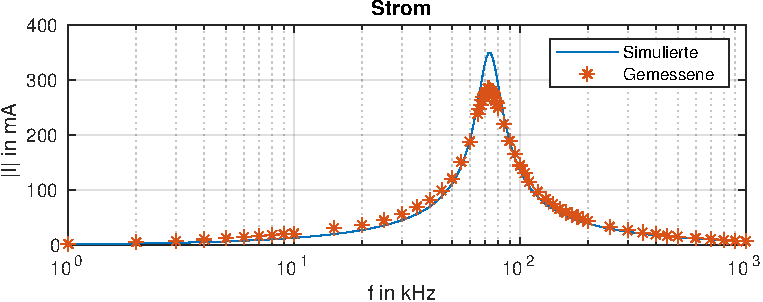
\includegraphics{src/stromimpedanzlab3.pdf}
    \caption{Strom anhängig von Frequenz}
    \label{fig:strom}
\end{figure}
\begin{figure}[H]
    \centering
    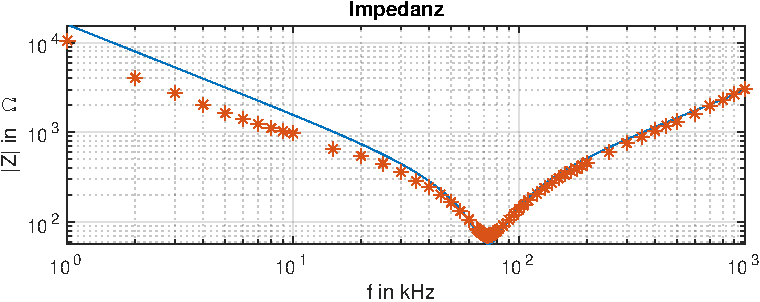
\includegraphics{src/impedanzlab3.pdf}
    \caption{Impedanz abhängig von Frequenz}
    \label{fig:impedanz}
\end{figure}

%
%
%
\begin{flushright}
  \textit{\autorA}
\end{flushright}
%
%------------------------------%
%------ Ende eures Teils ------%
%------------------------------%
%
%
%